\documentclass[aspectratio=169]{beamer}

\input{../slides-macros.tex}

\newif\ifmovies%
\moviestrue%
%\moviesfalse

\newif\ifsubs%
\substrue%
%\subsfalse

\newif\ifnotes%
\notestrue%
%\notesfalse

\begin{document}

%======================================================================
\begin{frame}\frametitle{}

\vspace*{0.3in}

\textrm{{\huge\bfseries\color{myOrange} Physics-informed neural networks to solve the compressible Euler equations}}

\vspace*{0.2in}
\hrule

%\begin{center}
%\includegraphics[width=0.15\textwidth]{Figures/ceesd-wordcloud.png}
%\end{center}
\hrule

\vspace*{0.1in}
\hfill\cPI{Dario Rodriguez} \rPI{(AE)}\\

\end{frame}
%======================================================================

%======================================================================
\begin{frame}\frametitle{Overview}

	\begin{itemize}
		\item Approximate solution of the Euler equations using a neural network (forward method)
	\end{itemize}
	
	\vspace{2mm}
	
	\begin{columns}
		\begin{column}{0.5\textwidth}			
			1-D Compressible Euler equations
			
			\begin{equation*}
				\frac{\partial U}{\partial t} + A \frac{\partial U}{\partial x} = 0
			\end{equation*}
			
			where,			
			\begin{align*}
				U = \left ( \rho, u, p \right)^T \\
				\vspace{10pt}
				A = \begin{bmatrix}
					u & \rho & 0 \\
					0 & u & \frac{1}{\rho} \\
					0 & \rho a^2 & u
				\end{bmatrix} \\
				a = \sqrt{\gamma p / \rho}
			\end{align*}
			
		\end{column}
		
		\begin{column}{0.5\textwidth}
			
			\begin{itemize}
				\item 2 inputs ($x$, $t$)
				\item 3 states outputs ($\rho$, $u$, $p$)
			\end{itemize}
			
			
			\begin{center}
				\includegraphics[width=1.\textwidth]{Figures/neural_network_architecture.png}
			\end{center}			
		\end{column}
	\end{columns}

\end{frame}
%======================================================================

%======================================================================
\begin{frame}\frametitle{Loss function}
	
	\begin{itemize}
		\item In general, the loss function is defined as follows:
	\end{itemize}

	\begin{gather*}
			L(\theta) = \frac{1}{N_f} \left | \frac{\partial \tilde{U}}{\partial t} (x,t,\theta) + \tilde{A} \frac{\partial \tilde{U}}{\partial x} (x, t, \theta) \right |^2_{\Omega \times (0, T]} + \\ \frac{1}{N_{IC}} \left | \tilde{U}(x, 0, \theta) - U(x, 0) \right |^2_{\Omega} + \frac{1}{N_{BC}} \left | \tilde{U}(x, t, \omega) - U(x,t) \right |^2_{\partial \Omega \times (o, T]}
	\end{gather*}
			
	\begin{itemize}
		\item Problem-specific $\rightarrow$ Sod shock tube problem
	\end{itemize}
	
	\begin{columns}
		\begin{column}{0.5\textwidth}
			\begin{equation*}
				\begin{bmatrix}
					\rho_L \\
					u_L \\
					P_L \\
				\end{bmatrix} = \begin{bmatrix}
					1.0 \\
					0.0 \\
					1.0 \\
				\end{bmatrix}
			\end{equation*}
		\end{column}
		
		
		\begin{column}{0.5\textwidth}
			\begin{equation*}
				\begin{bmatrix}
					\rho_L \\
					u_L \\
					P_L \\
				\end{bmatrix} = \begin{bmatrix}
					0.125 \\
					0.0 \\
					0.1 \\
				\end{bmatrix}
			\end{equation*}
		\end{column}	
	\end{columns}
	

\end{frame}
%======================================================================



%======================================================================
\begin{frame}\frametitle{Advances}
	
	A public repository \includegraphics[width=0.05\textwidth]{Figures/github_logo.png} \alert{\href{https://github.com/dalexa10/Machine_Learning/tree/main/5_Scientific_Machine_Learning/5_PINNs_Euler_Equations}{link}} was setup to host the models implemented
	
	\vspace{3mm}
	
	Four different models were trained by using a neural network (30-neuron width \& 7 hidden layers), a learning rate of 0.0005
	and the classical Adam optimizer. The epochs for these cases were set to 5000
		
	\begin{itemize}
		\item Space domain unaltered ($x \in [0, 1]$), no weights for losses
		\item Space domain extended ($x \in [-1.5, 3.125]$), no weights for losses
		\item Space domain unaltered ($x \in [0, 1]$), loss weights added (0.1 for PDE loss and 10 for IC loss)
		\item Space domain extended ($x \in [-1.5, 3.125]$), loss weights added (0.1 for PDE loss and 10 for IC loss)
	\end{itemize}
	

	
\end{frame}
%======================================================================


%======================================================================
\begin{frame}\frametitle{Preliminary results}
	\begin{itemize}
		\item The outcomes from the mentioned trained models are shown below.
		\item A comparison has been made only the exact solution at the desired time ($t=0.2$)
	\end{itemize}
	
	\begin{center}
		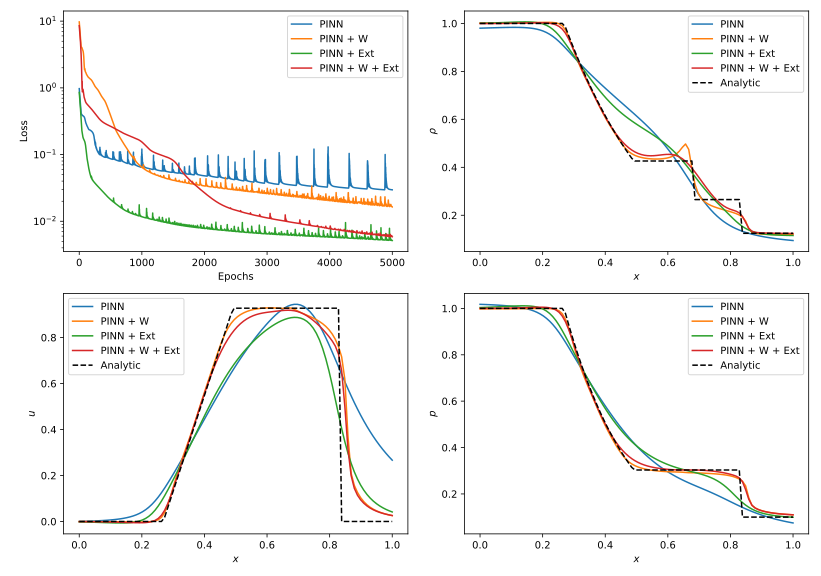
\includegraphics[width=0.65\textwidth]{Figures/preliminary_results.pdf}
	\end{center}
\end{frame}
%======================================================================


%======================================================================
\begin{frame}\frametitle{Difficulties \& Next steps}

	\begin{itemize}
		\item \textbf{\textcolor{myOrange}{Difficulties}}
			
			\begin{itemize}
				\item None of the models trained is able to completely capture the physics at the discontinuity (shock)
				\item Some models are presenting oscillations, while others present dissipation 
				\item So far, training the models using cpu-only machines requires significant time (for 5000 epoch $\approx$ 15[min])
			\end{itemize}
		
		\vspace{3mm}
		
		\item \textbf{\textcolor{myOrange}{Next steps}}
		
		\begin{itemize}
			\item Train the model using any GPU-accelerated device (HAL, local) and compare training times
			\item Implement a formal comparison with the exact solution and a high-order numerical method (WENO scheme)
			\item Define a set of neural networks parameters (width, hidden layers, optimizers, mini batches) and train the model with
			their combination. 
			\item For the previous goal, a shell script will be created to set the aforesaid parameters and run the jobs automatically
			in a remote computer		
			\item Implement either a 2-D compressible flow case or solve the inverse problem for a given set of density gradients (mimicking a Schlieren image)
		\end{itemize}	
		
	\end{itemize}

\end{frame}
%======================================================================

%======================================================================
\begin{frame}\frametitle{References}
	
	\begin{enumerate}
		\item Mao, Z., Jagtap, A. D., \& Karniadakis, G. E. (2020). Physics-informed neural networks for high-speed flows. Computer Methods in Applied Mechanics and Engineering, 360, 112789
		\item Papados, A. Solving hydrodynamic shock-tube problems using weighted physics-informed neural networks with domain extension.
	\end{enumerate}
	
\end{frame}
%======================================================================





\end{document}
